%%%%%%%%%%%%%%%%%%%%%%%%%%%%%%%%%%%%%%%%%%%%%%%%%%%%%%%%%%%%%%%%%%%%%%%%%%%%%%%%
%%%%%%%%%%%%%%%%%%%%%%%%%%%%%%%%%%%%%%%%%%%%%%%%%%%%%%%%%%%%%%%%%%%%%%%%%%%%%%%%
\clearpage
\section{Design development - control design}\label{sec:controller}
\tikzset{%
  block/.style    = {draw, thick, rectangle, minimum height = 3em,
    minimum width = 3em},
  sum/.style      = {draw, circle, node distance = 2cm}, % Adder
  input/.style    = {coordinate}, % Input
  output/.style   = {coordinate} % Output
}
%%%%%%%%%%%%%%%%%%%%%%%%%%%%%%%%%%%%%%%%%%%%%%%%%%%%%%%%%%%%%%%%%%%%%%%%%%%%%%%%
\subsection{Introduction}
Our system description works on the basis of a model perturbed from steady-state.
%%%%%%%%%%%%%%%%%%%%%%%%%%%%%%%%%%%%%%%%%%%%%%%%%%%%%%%%%%%%%%%%%%%%%%%%%%%%%%%%
\subsection{Open-loop: a model to estimate time-varying perturbations}
The block diagram for our open-loop perturbed system is provided in Figure~\ref{block:openloop}.
Thick lines denote vector quantities.
\begin{figure}[H]
\centering
\fbox{
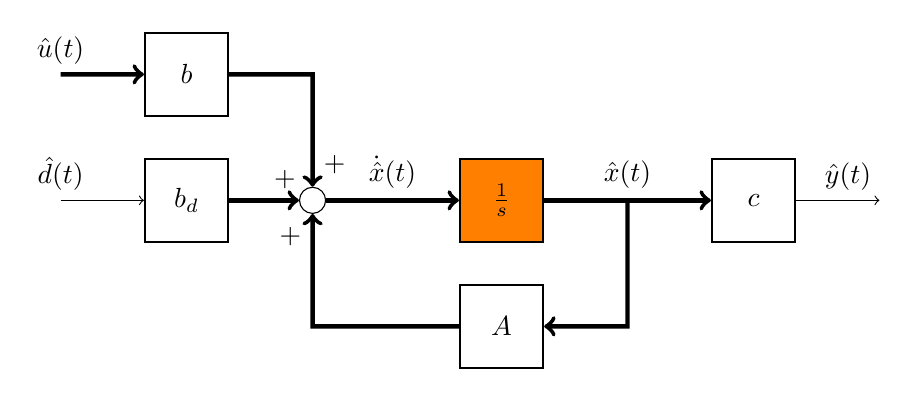
\begin{tikzpicture}[scale = 0.8]
%blocks
\draw
	(2,2) node [block] (bb) {$\boldsymbol{b}$}
	(4,0) node [sum] (s1) {\suma}
	(7,0) node [block, fill = orange] (i1) {$\frac{1}{s}$}
	(7,-2) node [block] (bA) {$\boldsymbol{A}$}
	(2,0) node [block] (bbD) {$\boldsymbol{b}_d$}
	(11,0) node [block] (bc) {$\boldsymbol{c}$};
%lines
\draw[->, ultra thick] (0,2) -- (bb);
\draw[->, ultra thick] (bb) -- (4,2) -- node [anchor = west, pos = 0.8] {$+$} (s1);
\draw[->, ultra thick] (s1) -- node [above] {$\dot{\hat{\boldsymbol{x}}}(t)$} (i1);
\draw[->, ultra thick] (i1) -- node [above] {$\hat{\boldsymbol{x}}(t)$} (bc);
\draw[->, ultra thick] (9,0) -- (9,-2) -- (bA);
\draw[->, ultra thick] (bA) -- (4,-2) -- node [anchor = east, pos = 0.8] {$+$} (s1);
\draw[->] (bc) -- (13,0);
%more lines
\draw[->] (0,0) -- (bbD);
\draw[->, ultra thick] (bbD) -- node [anchor = south, pos = 0.8] {$+$} (s1);
%labels
\coordinate[label = above:$\hat{\boldsymbol{u}}(t)$] (u) at (0,2);
\coordinate[label = above:$\hat{d}(t)$] (hatd) at (0,0);
\coordinate[label = above:$\hat{y}(t)$] (haty) at (12.5,0);
\end{tikzpicture}
}
\caption{}
\label{block:openloop}
\end{figure}
%%%%%%%%%%%%%%%%%%%%%%%%%%%%%%%%%%%%%%%%%%%%%%%%%%%%%%%%%%%%%%%%%%%%%%%%%%%%%%%%
%%%%%%%%%%%%%%%%%%%%%%%%%%%%%%%%%%%%%%%%%%%%%%%%%%%%%%%%%%%%%%%%%%%%%%%%%%%%%%%%
\subsection{Estimating voltages and currents for full-state feedback: the Luenberger observer}
For our system, there are states that are not able to be measured through any sensor regime (e.g. the voltages across ideal capacitors decoupled from parasitic resistances $v_{C1}$, $v_{C2}$). A Luenberger observer may be used to produce estimates of the system states, which may then be employed in a full-state feedback closed-loop control regime.
\newpar
A system is said to be observable (i.e. has no unobservable states) if the observability matrix as defined in Equation~(\ref{eqn:observable}) has full rank. This may easily be checked using the \textsf{MATLAB} call of~(\ref{matlab:observable}).
\begin{align}
\mathcal{O}
=
\begin{bmatrix}
\boldsymbol{c} \\
\boldsymbol{c}\boldsymbol{A} \\
\boldsymbol{c}\boldsymbol{A}^2 \\
\vdots \\
\boldsymbol{c}\boldsymbol{A}^{n - 1}
\end{bmatrix}
\qquad
\text{for a system with } n \text{ states}
\label{eqn:observable}
\end{align}
%
\begin{align}
\texttt{rank(obsv(A, c)) == 4}
\label{matlab:observable}
\end{align}
~\\
~\rule{\textwidth}{0.5pt}
\begin{align}
\boldsymbol{\dot{\hat{x}}}_\ell (t) &= \boldsymbol{A}\hat{\boldsymbol{x}}_\ell(t) + \boldsymbol{b}\hat{\boldsymbol{u}}(t) + \boldsymbol{b}_d \hat{d}(t) + \boldsymbol{L}\squarey{\hat{y}(t) - \hat{y}_\ell(t)}
\label{eqn:observer}
\\[11pt]
\boldsymbol{\dot{\hat{x}}}_\ell (t) &= \squarey{\boldsymbol{A} - \boldsymbol{L}\boldsymbol{c}}\hat{\boldsymbol{x}}_\ell(t) + \boldsymbol{b}\hat{\boldsymbol{u}}(t) + \boldsymbol{b}_d \hat{d}(t) + \boldsymbol{L}\hat{y}(t)
\label{eqn:observer2}
\end{align}
For an observable system, estimates of the perturbed plant states may be obtained by extracting the state vector in the system described according to Equation~(\ref{eqn:observer}) and the equivalent Equation~(\ref{eqn:observer2}), where
\begin{itemize}
\item $\boldsymbol{x}_\ell(t)$: vector containing state estimates
\item $y(t)$: measured converter circuit output voltage
\item $\hat{y}(t) = y(t) - Y$ where $Y$ is the steady-state output voltage as predicted by converter circuit model according to Equation~(\ref{eqn:modelY})
\item $\hat{\boldsymbol{u}}(t) = \boldsymbol{u}(t) - \boldsymbol{U} = \begin{bmatrix}v_g - V_g & 0 & 0 & 0\end{bmatrix}$ is measured in the converter circuit
\item $\boldsymbol{L}$: observer gain
\end{itemize}
If $\squarey{\boldsymbol{A} - \boldsymbol{L}\boldsymbol{c}}$ is stable, then the error between the estimated and actual system states decays to 0 exponentially.
\newpar
The observer gain matrix is typically populated such that the eigenvalues of $\boldsymbol{A} - \boldsymbol{L}\boldsymbol{c}$ are at least $10 \times$ faster than the eigenvalues of the closed-loop feedback system. The eigenvalues of this system may be placed by specifying the pole locations and calling \textsf{MATLAB}'s \texttt{acker} function as per~(\ref{matlab:place}).
\begin{align}
\texttt{L = acker(A', c', [p p p p])'}
\label{matlab:place}
\end{align}
where \texttt{p} is the desired pole location. Note that $(\quad\texttt{'}\quad)$ denotes transposition.
%%%%%%%%%%%%%%%%%%%%%%%%%%%%%%%%%%%%%%%%%%%%%%%%%%%%%%%%%%%%%%%%%%%%%%%%%%%%%%%%
The block diagram representation of Equation~(\ref{eqn:observer}) is given in Figure~\ref{block:observer}.
\begin{figure}[H]
\centering
\fbox{
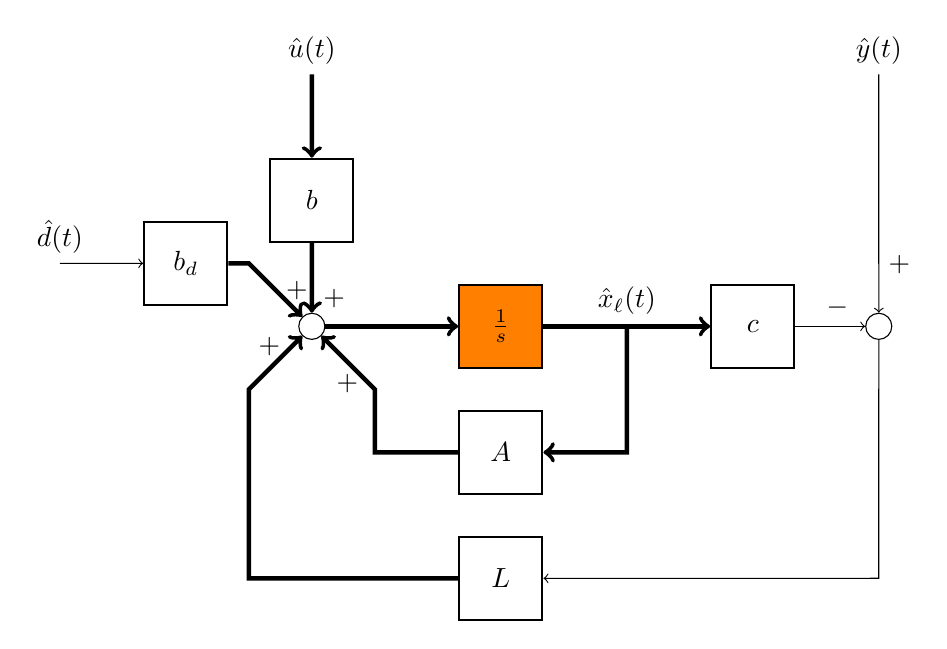
\begin{tikzpicture}[scale = 0.8]
%observer blocks
\draw
	(4,2) node [block] (bb) {$\boldsymbol{b}$}
	(4,0) node [sum] (s1) {\suma}
	(7,0) node [block, fill = orange] (i1) {$\frac{1}{s}$}
	(7,-2) node [block] (bA) {$\boldsymbol{A}$}
	(7,-4) node [block] (bL) {$\boldsymbol{L}$}
	(2,1) node [block] (bbD) {$\boldsymbol{b}_d$}
	(11,0) node [block] (bc) {$\boldsymbol{c}$};
%observer lines
\draw[->, ultra thick] (4,4) -- (bb);
\draw[->, ultra thick] (bb) -- node [anchor = west, pos = 0.8] {$+$} (s1);
\draw[->, ultra thick] (s1) -- (i1);
\draw[->, ultra thick] (i1) -- node [above] {$\hat{\boldsymbol{x}}_\ell(t)$} (bc);
\draw[->, ultra thick] (9,0) -- (9,-2) -- (bA);
\draw[->, ultra thick] (bA) -- (5,-2) -- (5,-1) -- node [anchor = east, pos = 0.1] {$+$} (s1);
\draw[->, ultra thick] (bbD) -- (3,1) -- node [anchor = south, pos = 0.9] {$+$} (s1);
%more observer blocks
\draw (13,0) node [sum] (sobserve) {\suma};
%more observer lines
\draw[->] (sobserve) -- (13,-4) -- (bL);
\draw[->, ultra thick] (bL) -- (3,-4) -- (3,-1) -- node [anchor = east, pos = 0.8] {$+$} (s1);
\draw[->] (bc) -- node [anchor = south, pos = 0.6] {$-$} (sobserve);
\draw[->] (13,4) -- node [anchor = west, pos = 0.8] {$+$} (sobserve);
\draw[->] (0,1) -- (bbD);
%signal labels
\coordinate[label = above:$\hat{d}(t)$] (d) at (0,1);
\coordinate[label = above:$\hat{\boldsymbol{u}}(t)$] (u) at (4,4);
\coordinate[label = above:$\hat{y}(t)$] (yhat) at (13,4);
\end{tikzpicture}
}
\caption{}
\label{block:observer}
\end{figure}
%%%%%%%%%%%%%%%%%%%%%%%%%%%%%%%%%%%%%%%%%%%%%%%%%%%%%%%%%%%%%%%%%%%%%%%%%%%%%%%%
The same system may be represented in a slightly different way that is of more relevance under discretisation. This different representation is provided in Figure~\ref{block:observer2}. Blocks to extract the true state estimate (i.e. sum of transient and steady-state) are introduced also. This system is described by Equation~(\ref{eqn:observer2}).
\begin{figure}[H]
\centering
\fbox{
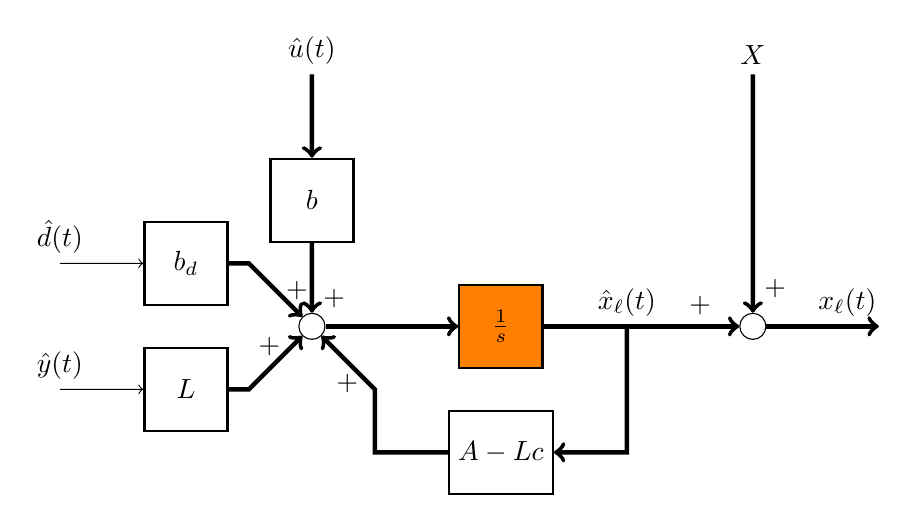
\begin{tikzpicture}[scale = 0.8]
%observer blocks
\draw
	(4,2) node [block] (bb) {$\boldsymbol{b}$}
	(4,0) node [sum] (s1) {\suma}
	(7,0) node [block, fill = orange] (i1) {$\frac{1}{s}$}
	(7,-2) node [block] (bA) {$\boldsymbol{A} - \boldsymbol{L}\boldsymbol{c}$}
	(2,-1) node [block] (bL) {$\boldsymbol{L}$}
	(2,1) node [block] (bbD) {$\boldsymbol{b}_d$}
	(11,0) node [sum] (s2) {\suma};
%observer lines
\draw[->, ultra thick] (4,4) -- (bb);
\draw[->, ultra thick] (bb) -- node [anchor = west, pos = 0.8] {$+$} (s1);
\draw[->, ultra thick] (s1) -- (i1);
\draw[->, ultra thick] (i1) -- node [anchor = south, pos = 0.8] {$+$} (s2);
\draw[->, ultra thick] (9,0) -- (9,-2) -- (bA);
\draw[->, ultra thick] (bA) -- (5,-2) -- (5,-1) -- node [anchor = east, pos = 0.1] {$+$} (s1);
\draw[->, ultra thick] (bbD) -- (3,1) -- node [anchor = south, pos = 0.9] {$+$} (s1);
%more observer lines
\draw[->, ultra thick] (bL) -- (3,-1) -- node [anchor = east, pos = 0.8] {$+$} (s1);
\draw[->] (0,1) -- (bbD);
\draw[->] (0,-1) -- (bL);
\draw[->, ultra thick] (11,4) -- node [anchor = west, pos = 0.9] {$+$} (s2);
\draw[->, ultra thick] (s2) -- (13,0);
%signal labels
\coordinate[label = above:$\hat{d}(t)$] (d) at (0,1);
\coordinate[label = above:$\hat{\boldsymbol{u}}(t)$] (u) at (4,4);
\coordinate[label = above:$\hat{y}(t)$] (yhat) at (0,-1);
\coordinate[label = above:$\boldsymbol{X}$] (bigx) at (11,4);
\coordinate[label = above:$\boldsymbol{x}_\ell(t)$] (smallx) at (12.5,0);
\coordinate[label = above:$\hat{\boldsymbol{x}}_\ell(t)$] (hatx) at (9,0);
\end{tikzpicture}
}
\caption{}
\label{block:observer2}
\end{figure}
The state vector $\boldsymbol{x}_l (t)$ contains the estimates of the internal system states, while $\hat{\boldsymbol{x}}_l (t)$ may be fed back under full-state feedback to achieve desirable closed-loop performance.
%%%%%%%%%%%%%%%%%%%%%%%%%%%%%%%%%%%%%%%%%%%%%%%%%%%%%%%%%%%%%%%%%%%%%%%%%%%%%%%%
%%%%%%%%%%%%%%%%%%%%%%%%%%%%%%%%%%%%%%%%%%%%%%%%%%%%%%%%%%%%%%%%%%%%%%%%%%%%%%%%
\subsection{Closing the loop: observer state feedback}
\begin{figure}[H]
\centering
\fbox{
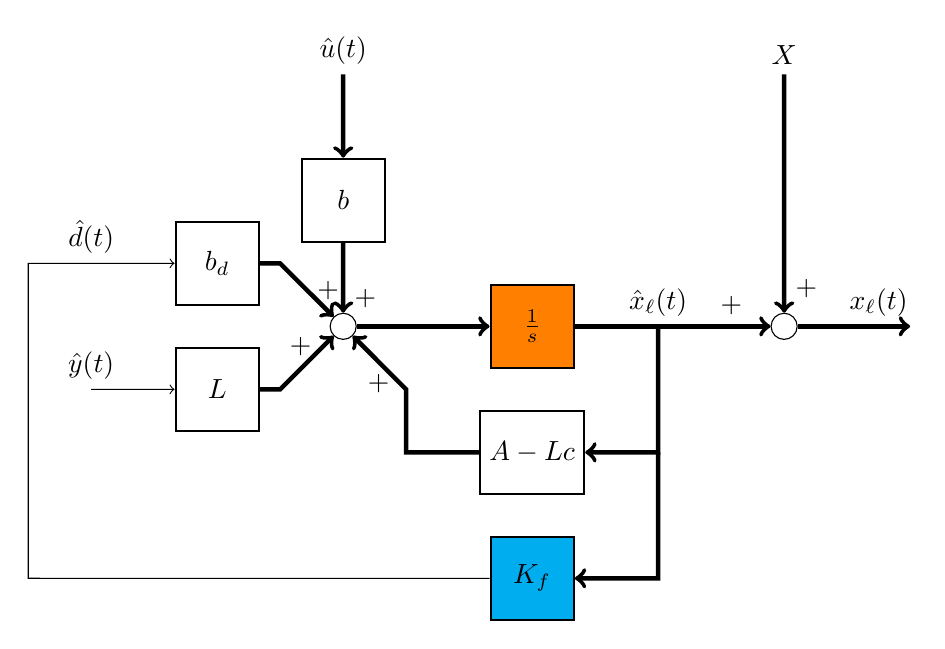
\begin{tikzpicture}[scale = 0.8]
% blocks
\draw
	(4,2) node [block] (bb) {$\boldsymbol{b}$}
	(4,0) node [sum] (s1) {\suma}
	(7,0) node [block, fill = orange] (i1) {$\frac{1}{s}$}
	(7,-2) node [block] (bA) {$\boldsymbol{A} - \boldsymbol{L}\boldsymbol{c}$}
	(2,-1) node [block] (bL) {$\boldsymbol{L}$}
	(2,1) node [block] (bbD) {$\boldsymbol{b}_d$}
	(11,0) node [sum] (s2) {\suma}
	(7,-4) node [block, fill = cyan] (bKf) {$\minus \boldsymbol{K}_f$};
% observer lines
\draw[->, ultra thick] (4,4) -- (bb);
\draw[->, ultra thick] (bb) -- node [anchor = west, pos = 0.8] {$+$} (s1);
\draw[->, ultra thick] (s1) -- (i1);
\draw[->, ultra thick] (i1) -- node [anchor = south, pos = 0.8] {$+$} (s2);
\draw[->, ultra thick] (9,0) -- (9,-2) -- (bA);
\draw[->, ultra thick] (bA) -- (5,-2) -- (5,-1) -- node [anchor = east, pos = 0.1] {$+$} (s1);
\draw[->, ultra thick] (bbD) -- (3,1) -- node [anchor = south, pos = 0.9] {$+$} (s1);
% more observer lines
\draw[->, ultra thick] (bL) -- (3,-1) -- node [anchor = east, pos = 0.8] {$+$} (s1);
\draw[->] (0,-1) -- (bL);
\draw[->, ultra thick] (11,4) -- node [anchor = west, pos = 0.9] {$+$} (s2);
\draw[->, ultra thick] (s2) -- (13,0);
% signal labels
\coordinate[label = above:$\hat{d}(t)$] (d) at (0,1);
\coordinate[label = above:$\hat{\boldsymbol{u}}(t)$] (u) at (4,4);
\coordinate[label = above:$\hat{y}(t)$] (yhat) at (0,-1);
\coordinate[label = above:$\boldsymbol{X}$] (bigx) at (11,4);
\coordinate[label = above:$\boldsymbol{x}_\ell(t)$] (smallx) at (12.5,0);
\coordinate[label = above:$\hat{\boldsymbol{x}}_\ell(t)$] (hatx) at (9,0);
% feedback lines
\draw[->, ultra thick] (9,-2) -- (9,-4) -- (bKf);
\draw[->] (bKf) -- (-1,-4) -- (-1,1) -- (bbD);
\end{tikzpicture}
}
\caption{}
\label{block:feedback}
\end{figure}
The gain matrix $\boldsymbol{K}_f$ is populated to produce desirable closed-loop performance. The non-zero steady-state error resulting from this scheme may be eliminated by introducing a reference input and integral action.
%%%%%%%%%%%%%%%%%%%%%%%%%%%%%%%%%%%%%%%%%%%%%%%%%%%%%%%%%%%%%%%%%%%%%%%%%%%%%%%%
%%%%%%%%%%%%%%%%%%%%%%%%%%%%%%%%%%%%%%%%%%%%%%%%%%%%%%%%%%%%%%%%%%%%%%%%%%%%%%%%
\subsection{Introducing a reference input and integral action}
\begin{figure}[H]
\centering
\fbox{
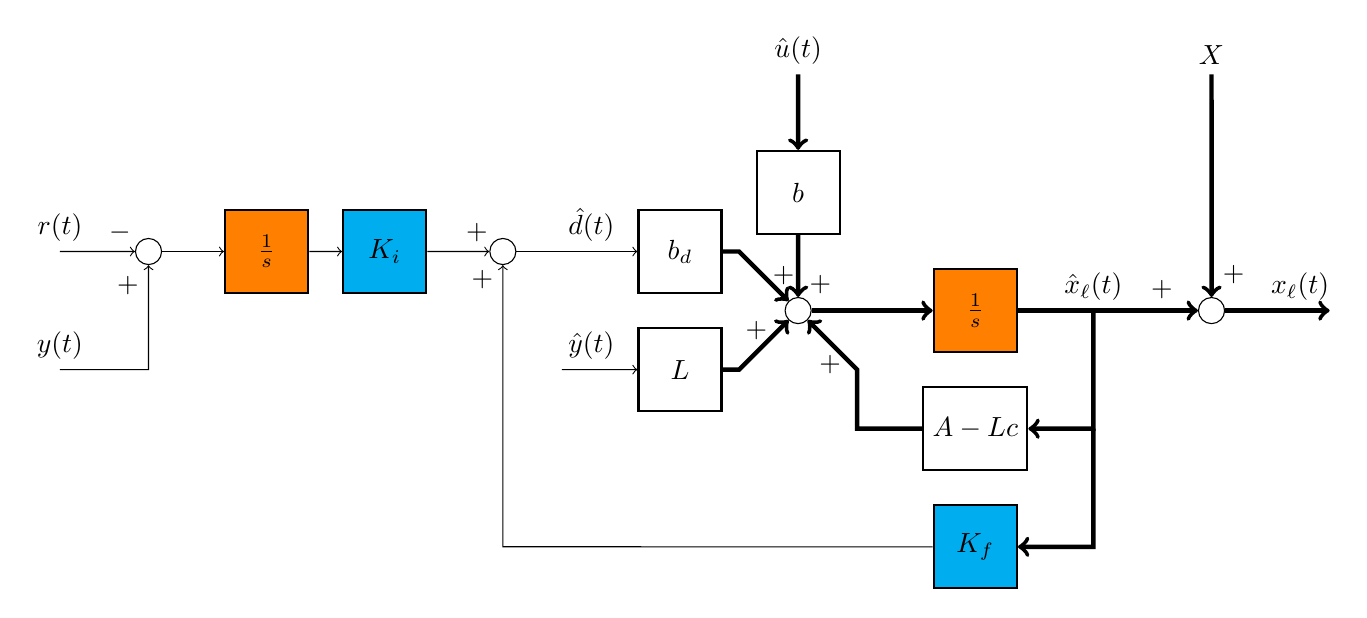
\begin{tikzpicture}[scale = 0.75]
% blocks
\draw
	(4,2) node [block] (bb) {$\boldsymbol{b}$}
	(4,0) node [sum] (s1) {\suma}
	(7,0) node [block, fill = orange] (i1) {$\frac{1}{s}$}
	(7,-2) node [block] (bA) {$\boldsymbol{A} - \boldsymbol{L}\boldsymbol{c}$}
	(2,-1) node [block] (bL) {$\boldsymbol{L}$}
	(2,1) node [block] (bbD) {$\boldsymbol{b}_d$}
	(11,0) node [sum] (s2) {\suma}
	(7,-4) node [block, fill = cyan] (bKf) {$\minus \boldsymbol{K}_f$};
% observer lines
\draw[->, ultra thick] (4,4) -- (bb);
\draw[->, ultra thick] (bb) -- node [anchor = west, pos = 0.8] {$+$} (s1);
\draw[->, ultra thick] (s1) -- (i1);
\draw[->, ultra thick] (i1) -- node [anchor = south, pos = 0.8] {$+$} (s2);
\draw[->, ultra thick] (9,0) -- (9,-2) -- (bA);
\draw[->, ultra thick] (bA) -- (5,-2) -- (5,-1) -- node [anchor = east, pos = 0.1] {$+$} (s1);
\draw[->, ultra thick] (bbD) -- (3,1) -- node [anchor = south, pos = 0.9] {$+$} (s1);
% more observer lines
\draw[->, ultra thick] (bL) -- (3,-1) -- node [anchor = east, pos = 0.8] {$+$} (s1);
\draw[->] (0,-1) -- (bL);
\draw[->, ultra thick] (11,4) -- node [anchor = west, pos = 0.9] {$+$} (s2);
\draw[->, ultra thick] (s2) -- (13,0);
% signal labels
\coordinate[label = above:$\hat{d}(t)$] (d) at (0.5,1);
\coordinate[label = above:$\hat{\boldsymbol{u}}(t)$] (u) at (4,4);
\coordinate[label = above:$\hat{y}(t)$] (yhat) at (0.5,-1);
\coordinate[label = above:$\boldsymbol{X}$] (bigx) at (11,4);
\coordinate[label = above:$\boldsymbol{x}_\ell(t)$] (smallx) at (12.5,0);
\coordinate[label = above:$\hat{\boldsymbol{x}}_\ell(t)$] (hatx) at (9,0);
\coordinate[label = above:$r(t)$] (r) at (-8.5,1);
\coordinate[label = above:$y(t)$] (r) at (-8.5,-1);
% integrator blocks
\draw
    (-1,1) node [sum] (s5) {\suma}
	(-3,1) node [block, fill = cyan] (bKi) {$\minus K_i$}
	(-5,1) node [block, fill = orange] (i2) {$\frac{1}{s}$}
	(-7,1) node [sum] (s4) {\suma};
% feedback lines
\draw[->, ultra thick] (9,-2) -- (9,-4) -- (bKf);
\draw[->] (bKf) -- (-1,-4) -- node [anchor = east, pos = 0.95] {$+$} (s5);
\draw[->] (s5) -- (bbD);
% integrator lines
\draw[->] (-8.5,1) -- node [anchor = south, pos = 0.8] {$-$} (s4);
\draw[->] (s4) -- (i2);
\draw[->] (i2) -- (bKi);
\draw[->] (bKi) -- node [anchor = south, pos = 0.8] {$+$} (s5);
\draw[->] (-8.5,-1) -- (-7,-1) -- node [anchor = east, pos = 0.8] {$+$} (s4);
\end{tikzpicture}
}
\caption{}
\label{block:integral}
\end{figure}
So our microcontroller will estimate the above system and send to the converter a PWM signal of duty ratio $d(t) = \hat{d}(t) + D$ where $D$ is the steady-state duty ratio used in generating a linear model of the system.
%%%%%%%%%%%%%%%%%%%%%%%%%%%%%%%%%%%%%%%%%%%%%%%%%%%%%%%%%%%%%%%%%%%%%%%%%%%%%%%%
\newpar
Our system description may be updated by augmenting the state vector with an additional state for the integral of the error $\dot{x}_i(t) = e(t) = y(t) - r(t)$ ($x_i(t) = \int \mathrm{d}t \curly{e(t)}$). Then
\begin{align*}
\boldsymbol{\dispdot[0mu]{\hat{x}}_a}(t) &= \boldsymbol{A}_a\hat{\boldsymbol{x}}_a(t) + \boldsymbol{b}_a \hat{\boldsymbol{u}}_a(t) + \boldsymbol{b}_{d_a} \hat{d}(t) + \boldsymbol{r}(t)
\\[11pt]
\hat{y}(t) &= \boldsymbol{c}_a \hat{\boldsymbol{x}}_a(t)
\end{align*}
and
\begingroup
\allowdisplaybreaks
\begin{align}
\boldsymbol{x}_a &=
\begin{bmatrix}
\hat{v}_{C1} & \hat{v}_{C2} & \hat{i}_{L1} & \hat{i}_{L2} & x_i
\end{bmatrix}^\intercal
\\[11pt]
\boldsymbol{u}_a &=
\begin{bmatrix}
v_g - V_g & 0 & 0 & 0 & 0
\end{bmatrix}^\intercal
\\[11pt]
\boldsymbol{r}(t) &=
\begin{bmatrix}
0 & 0 & 0 & 0 & \minus r(t)
\end{bmatrix}^\intercal
\\[11pt]
\boldsymbol{A}_a &=
\begin{bmatrix}
\boldsymbol{A} & 0\\
\boldsymbol{c} & 0
\end{bmatrix}
\label{eqn:augmentedA}
\\[11pt]
\boldsymbol{b}_a
&=
\begin{bmatrix}
\boldsymbol{b} \\ 0
\end{bmatrix}
\\[11pt]
\boldsymbol{b}_{d_a}
&=
\begin{bmatrix}
\boldsymbol{b}_d \\ 0
\end{bmatrix}
\label{eqn:augmentedbD}
\\[11pt]
\boldsymbol{c}_a
&=
\begin{bmatrix}
\boldsymbol{c} & 0
\end{bmatrix}
\end{align}
\endgroup
%%%%%%%%%%%%%%%%%%%%%%%%%%%%%%%%%%%%%%%%%%%%%%%%%%%%%%%%%%%%%%%%%%%%%%%%%%%%%%%%
%%%%%%%%%%%%%%%%%%%%%%%%%%%%%%%%%%%%%%%%%%%%%%%%%%%%%%%%%%%%%%%%%%%%%%%%%%%%%%%%
\subsection{Linear quadratic regulator (LQR); a method for determining $\boldsymbol{K}_f$ and $K_i$}\label{sec:LQR}
\textsf{MATLAB}'s \texttt{lqr} function was used to compute the gains $\boldsymbol{K}_f$ and $K_i$. This function is called with arguments \texttt{(A, B, Q, R, N)}, which are used to generated the state feedback law $\boldsymbol{u} = -\boldsymbol{K}\boldsymbol{x}$ that minimises the quadratic cost function
\begin{align}
J = \int_0^\infty \mathrm{d}t\curly{\boldsymbol{x}^\intercal \boldsymbol{Q} \boldsymbol{x}
+ \boldsymbol{u}^\intercal \boldsymbol{R} \boldsymbol{u}
+ 2 \boldsymbol{x}^\intercal \boldsymbol{N} \boldsymbol{u}}
\label{eqn:LQR}
\end{align}
subject to system dynamics
\begin{align*}
\boldsymbol{\dot{x}} = \boldsymbol{A}\boldsymbol{x} + \boldsymbol{B}\boldsymbol{u}
\end{align*}
and the conditions
\begin{itemize}
    \item $(\boldsymbol{A}, \, \boldsymbol{B})$ is stabilizable\footnote{definition: all uncontrollable states are bounded; our system has no uncontrollable states and so is stabilizable} from \texttt{u}
    \item $0 < \boldsymbol{R}$
\end{itemize}
For our purposes the \texttt{lqr} function is called as
\begin{align*}
\texttt{lqr(A\_a, bD\_a, w*q, r)}
\end{align*}
where, for our system
\begin{itemize}
	\item $\texttt{A\_a}$: $\boldsymbol{A}_a$ of Equation~\ref{eqn:augmentedA}
	\item $\texttt{bD\_a}$: $\boldsymbol{b}_{d_a}$ of Equation~\ref{eqn:augmentedbD}
	\item $w \in \Re$: scalar multiplicative factor of $q$
	\item $q\in \Re^{5 \times 5}$: $\boldsymbol{Q}$ of Equation~\ref{eqn:LQR}; diagonal positive definite weight matrix that penalises variation of states from desired value
	\item $r \in \Re$: $\boldsymbol{R}$ of Equation~\ref{eqn:LQR}; weight that penalises control effort
	\item $N = 0$
\end{itemize}
$\boldsymbol{K}$ is extracted as
\begin{align*}
\boldsymbol{K}
=
\begin{bmatrix}
\boldsymbol{K}_f & K_i
\end{bmatrix}
=
\boldsymbol{R}^{\minus 1} \paren{\boldsymbol{B}^\intercal \boldsymbol{S} + \boldsymbol{N}^\intercal}
\end{align*}
where $\boldsymbol{S}$ is the solution to the algebraic Riccati equation
\begin{align*}
\boldsymbol{A}^\intercal \boldsymbol{S} + \boldsymbol{S}\boldsymbol{A} - \paren{\boldsymbol{S}\boldsymbol{B} + \boldsymbol{N}}\boldsymbol{R}^{\minus 1} \paren{\boldsymbol{B}^\intercal \boldsymbol{S} + \boldsymbol{N}^\intercal} + \boldsymbol{Q} = 0
\end{align*}
%%%%%%%%%%%%%%%%%%%%%%%%%%%%%%%%%%%%%%%%%%%%%%%%%%%%%%%%%%%%%%%%%%%%%%%%%%%%%%%%
%%%%%%%%%%%%%%%%%%%%%%%%%%%%%%%%%%%%%%%%%%%%%%%%%%%%%%%%%%%%%%%%%%%%%%%%%%%%%%%%
\subsection{Discretisation: achieving emulation of a continuous-time system on a discrete-time microprocessor}\label{sec:disc}
The control theory thus far has operated in the continuous-time domain. For implementation of our control algorithm on the microcontroller, the observer system and integral action must be discretised. The appropriate discretisation method for our system is `zero-order hold' (ZOH). In this method the control inputs ($\hat{d}(t)$, $\hat{\boldsymbol{u}}(t)$, $y(t)$, and $\hat{y}(t)$) are assumed to be constant over the sampling period $T_s$.
%%%%%%%%%%%%%%%%%%%%%%%%%%%%%%%%%%%%%%%%%%%%%%%%%%%%%%%%%%%%%%%%%%%%%%%%%%%%%%%%
\subsubsection{Discretising the observer - ZOH}
Our observer system has the following description
\begin{align*}
\boldsymbol{\dot{\hat{x}}}_\ell (t) = \squarey{\boldsymbol{A} - \boldsymbol{L}\boldsymbol{c}}\hat{\boldsymbol{x}}_\ell(t) + \boldsymbol{b}\hat{\boldsymbol{u}}(t) + \boldsymbol{b}_d \hat{d}(t) + \boldsymbol{L}\hat{y}(t)
\end{align*}
where
\begin{itemize}
\item $\hat{\boldsymbol{x}}_\ell(t)$: state vector produced by observer (estimated values)
\item $\hat{y}(t) = y(t) - Y$: output perturbation (measured output subtract steady-state output)
\end{itemize}
% \newpar
Assuming ZOH with a sampling time $T_s = \sfrac{1}{f_\text{sample}}$, the observer is described  by
\begin{align*}
\hat{\boldsymbol{x}}_\ell [k + 1] &= \overline{\squarey{\boldsymbol{A} - \boldsymbol{L}\boldsymbol{c}}}\hat{\boldsymbol{x}}_\ell[k] + \overline{\boldsymbol{b}}\hat{\boldsymbol{u}}[k] + \overline{\boldsymbol{b}_d} \hat{d}[k] + \overline{\boldsymbol{L}}\hat{y}[k]
\end{align*}
where
\begin{align*}
\overline{\squarey{\boldsymbol{A} - \boldsymbol{L}\boldsymbol{c}}} &= \exp \squarey{\paren{\boldsymbol{A} - \boldsymbol{L}\boldsymbol{c}}T_s}
\\[11pt]
\overline{\boldsymbol{b}} &= \paren{\int_0^{T_s} \mathrm{d}\tau \curly{\exp \squarey{\paren{\boldsymbol{A} - \boldsymbol{L}\boldsymbol{c}}\tau}}}\boldsymbol{b}
\\[11pt]
&= \paren{\boldsymbol{A} - \boldsymbol{L}\boldsymbol{c}}^{-1}
\paren{\overline{\squarey{\boldsymbol{A} - \boldsymbol{L}\boldsymbol{c}}} - \boldsymbol{I}_4}
\boldsymbol{b}
\\[11pt]
\overline{\boldsymbol{b}_d} &=
\paren{\boldsymbol{A} - \boldsymbol{L}\boldsymbol{c}}^{-1}
\paren{\overline{\squarey{\boldsymbol{A} - \boldsymbol{L}\boldsymbol{c}}} - \boldsymbol{I}_4}
\boldsymbol{b}_d
\\[11pt]
\overline{\boldsymbol{L}} &=
\paren{\boldsymbol{A} - \boldsymbol{L}\boldsymbol{c}}^{-1}
\paren{\overline{\squarey{\boldsymbol{A} - \boldsymbol{L}\boldsymbol{c}}} - \boldsymbol{I}_4}
\boldsymbol{L}
\end{align*}
and where $\boldsymbol{I}_4$ is the identity matrix of dimension 4.
\newpar
The block diagram of the ZOH-discretised observer is provided in Figure~\ref{block:observer_discrete}.
\begin{figure}[H]
\centering
\fbox{
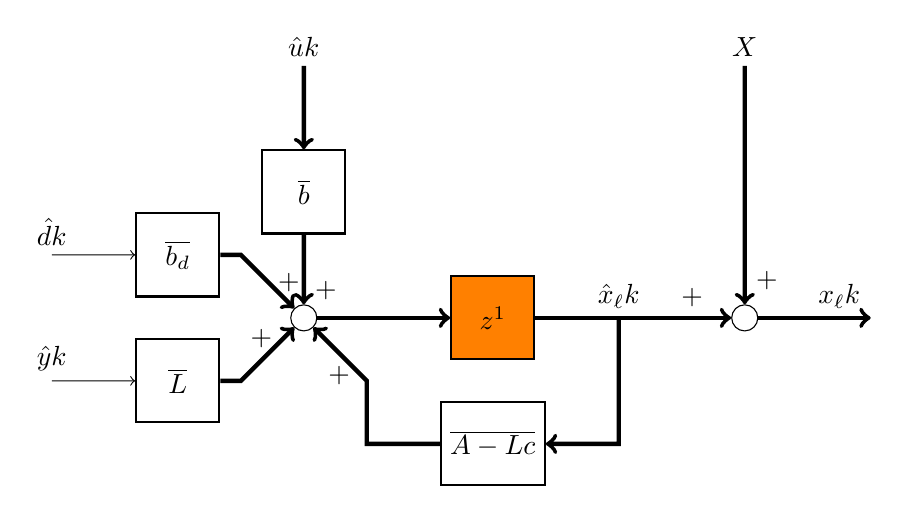
\begin{tikzpicture}[scale = 0.8]
%observer blocks
\draw
	(4,2) node [block] (bb) {$\overline{\boldsymbol{b}}$}
	(4,0) node [sum] (s1) {\suma}
	(7,0) node [block, fill = orange] (i1) {$z^{\minus 1}$}
	(7,-2) node [block] (bA) {$\overline{\squarey{\boldsymbol{A} - \boldsymbol{L}\boldsymbol{c}}}$}
	(2,-1) node [block] (bL) {$\overline{\boldsymbol{L}}$}
	(2,1) node [block] (bbD) {$\overline{\boldsymbol{b}_d}$}
	(11,0) node [sum] (s2) {\suma};
%observer lines
\draw[->, ultra thick] (4,4) -- (bb);
\draw[->, ultra thick] (bb) -- node [anchor = west, pos = 0.8] {$+$} (s1);
\draw[->, ultra thick] (s1) -- (i1);
\draw[->, ultra thick] (i1) -- node [anchor = south, pos = 0.8] {$+$} (s2);
\draw[->, ultra thick] (9,0) -- (9,-2) -- (bA);
\draw[->, ultra thick] (bA) -- (5,-2) -- (5,-1) -- node [anchor = east, pos = 0.1] {$+$} (s1);
\draw[->, ultra thick] (bbD) -- (3,1) -- node [anchor = south, pos = 0.9] {$+$} (s1);
%more observer lines
\draw[->, ultra thick] (bL) -- (3,-1) -- node [anchor = east, pos = 0.8] {$+$} (s1);
\draw[->] (0,1) -- (bbD);
\draw[->] (0,-1) -- (bL);
\draw[->, ultra thick] (11,4) -- node [anchor = west, pos = 0.9] {$+$} (s2);
\draw[->, ultra thick] (s2) -- (13,0);
%signal labels
\coordinate[label = above:$\hat{d}\squarey{k}$] (d) at (0,1);
\coordinate[label = above:$\hat{\boldsymbol{u}}\squarey{k}$] (u) at (4,4);
\coordinate[label = above:$\hat{y}\squarey{k}$] (yhat) at (0,-1);
\coordinate[label = above:$\boldsymbol{X}$] (bigx) at (11,4);
\coordinate[label = above:$\boldsymbol{x}_\ell\squarey{k}$] (smallx) at (12.5,0);
\coordinate[label = above:$\hat{\boldsymbol{x}}_\ell\squarey{k}$] (hatx) at (9,0);
\end{tikzpicture}
}
\caption{}
\label{block:observer_discrete}
\end{figure}
%%%%%%%%%%%%%%%%%%%%%%%%%%%%%%%%%%%%%%%%%%%%%%%%%%%%%%%%%%%%%%%%%%%%%%%%%%%%%%%%
\subsubsection{Discretising integral action - forward-euler integration}
Discrete time integral action under the forward-euler method is achieved through the transfer function of Equation~\ref{eqn:integral_discrete}
\begin{align}\label{eqn:integral_discrete}
H(z) = \frac{T_s}{z - 1}
\end{align}
%%%%%%%%%%%%%%%%%%%%%%%%%%%%%%%%%%%%%%%%%%%%%%%%%%%%%%%%%%%%%%%%%%%%%%%%%%%%%%%%
\subsubsection{Augmented control loop - discrete time}\label{sec:control_ultimate}
The block diagram for the resulting fully-discrete control loop is given in Figure~\ref{block:control_discrete}.
\begin{figure}[H]
\centering
\fbox{
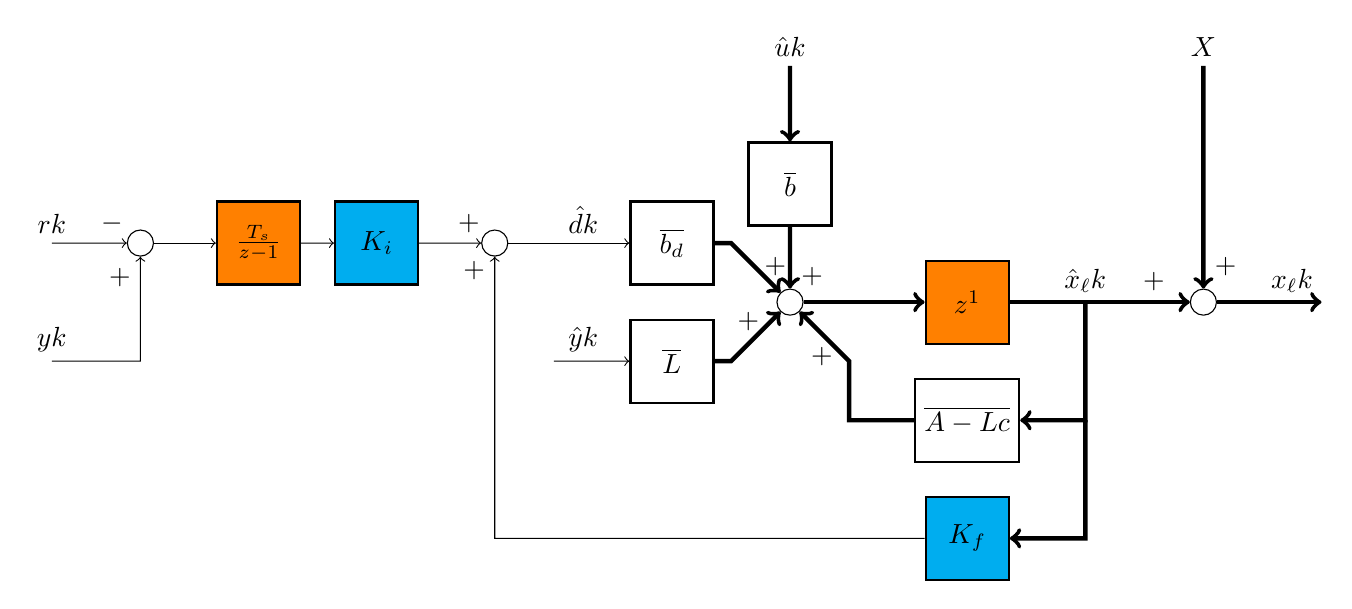
\begin{tikzpicture}[scale = 0.75]
% blocks
\draw
	(4,2) node [block] (bb) {$\overline{\boldsymbol{b}}$}
	(4,0) node [sum] (s1) {\suma}
	(7,0) node [block, fill = orange] (i1) {$z^{\minus 1}$}
	(7,-2) node [block] (bA) {$\overline{\squarey{\boldsymbol{A} - \boldsymbol{L}\boldsymbol{c}}}$}
	(2,-1) node [block] (bL) {$\overline{\boldsymbol{L}}$}
	(2,1) node [block] (bbD) {$\overline{\boldsymbol{b}_d}$}
	(11,0) node [sum] (s2) {\suma}
	(7,-4) node [block, fill = cyan] (bKf) {$\minus \boldsymbol{K}_f$};
% observer lines
\draw[->, ultra thick] (4,4) -- (bb);
\draw[->, ultra thick] (bb) -- node [anchor = west, pos = 0.8] {$+$} (s1);
\draw[->, ultra thick] (s1) -- (i1);
\draw[->, ultra thick] (i1) -- node [anchor = south, pos = 0.8] {$+$} (s2);
\draw[->, ultra thick] (9,0) -- (9,-2) -- (bA);
\draw[->, ultra thick] (bA) -- (5,-2) -- (5,-1) -- node [anchor = east, pos = 0.1] {$+$} (s1);
\draw[->, ultra thick] (bbD) -- (3,1) -- node [anchor = south, pos = 0.9] {$+$} (s1);
% more observer lines
\draw[->, ultra thick] (bL) -- (3,-1) -- node [anchor = east, pos = 0.8] {$+$} (s1);
\draw[->] (0,-1) -- (bL);
\draw[->, ultra thick] (11,4) -- node [anchor = west, pos = 0.9] {$+$} (s2);
\draw[->, ultra thick] (s2) -- (13,0);
% signal labels
\coordinate[label = above:$\hat{d}\squarey{k}$] (d) at (0.5,1);
\coordinate[label = above:$\hat{\boldsymbol{u}}\squarey{k}$] (u) at (4,4);
\coordinate[label = above:$\hat{y}\squarey{k}$] (yhat) at (0.5,-1);
\coordinate[label = above:$\boldsymbol{X}$] (bigx) at (11,4);
\coordinate[label = above:$\boldsymbol{x}_\ell\squarey{k}$] (smallx) at (12.5,0);
\coordinate[label = above:$\hat{\boldsymbol{x}}_\ell\squarey{k}$] (hatx) at (9,0);
\coordinate[label = above:$r\squarey{k}$] (r) at (-8.5,1);
\coordinate[label = above:$y\squarey{k}$] (r) at (-8.5,-1);
% integrator blocks
\draw
    (-1,1) node [sum] (s5) {\suma}
	(-3,1) node [block, fill = cyan] (bKi) {$\minus K_i$}
	(-5,1) node [block, fill = orange] (i2) {$\frac{T_s}{z - 1}$}
	(-7,1) node [sum] (s4) {\suma};
% feedback lines
\draw[->, ultra thick] (9,-2) -- (9,-4) -- (bKf);
\draw[->] (bKf) -- (-1,-4) -- node [anchor = east, pos = 0.95] {$+$} (s5);
\draw[->] (s5) -- (bbD);
% integrator lines
\draw[->] (-8.5,1) -- node [anchor = south, pos = 0.8] {$-$} (s4);
\draw[->] (s4) -- (i2);
\draw[->] (i2) -- (bKi);
\draw[->] (bKi) -- node [anchor = south, pos = 0.8] {$+$} (s5);
\draw[->] (-8.5,-1) -- (-7,-1) -- node [anchor = east, pos = 0.8] {$+$} (s4);
\end{tikzpicture}
}
\caption{}
\label{block:control_discrete}
\end{figure}
%%%%%%%%%%%%%%%%%%%%%%%%%%%%%%%%%%%%%%%%%%%%%%%%%%%%%%%%%%%%%%%%%%%%%%%%%%%%%%%%
\subsubsection{Control summary}
At integer time step $k$:
\begin{itemize}
\item $r\squarey{k}$: input reference signal/desired output voltage
\item $y\squarey{k}$: output voltage as measured by ADC
\item $\hat{d}\squarey{k}$: duty ratio perturbation to be sent to update PWM signal
\item $\hat{y}\squarey{k}$: output voltage perturbation from steady-state calculated according to
    \begin{itemize}
    \item $\hat{y}\squarey{k} = y\squarey{k} - \, Y$
    \end{itemize}
\item $\hat{\boldsymbol{u}}\squarey{k}$: input vector perturbation from steady-state calculated according to
    \begin{itemize}
    \item $\hat{\boldsymbol{u}}\squarey{k} = \boldsymbol{u}\squarey{k} - \, \boldsymbol{U}$
    \item note that only the first element of $\hat{\boldsymbol{u}}\squarey{k}$ changes while running the control loop; diode forward voltage drop is considered to be unchanging under forward bias
    \end{itemize}
\item $\hat{\boldsymbol{x}}_\ell\squarey{k}$: estimated state vector perturbation from steady-state
    \begin{itemize}
    \item used for full-state feedback control
    \end{itemize}
\item $\boldsymbol{x}_\ell\squarey{k}$: estimated state vector
    \begin{itemize}
    \item vector containing estimates of state variables
    \end{itemize}
\end{itemize}
%%%%%%%%%%%%%%%%%%%%%%%%%%%%%%%%%%%%%%%%%%%%%%%%%%%%%%%%%%%%%%%%%%%%%%%%%%%%%%%%
\subsubsection{Physical realisation of our control loop}\label{sec:hardware_for_control}
The basic modules required for hardware implementation of our control loop will be introduced presently.
\paragraph{Measuring $v_g(t)$ and $y(t)$: op-amp sensing circuitry}
\paragraph{Writing the control signal to the DC-DC converter: achieving PWM functionality in hardware}
\paragraph{Iterating the control loop: using a microcontroller to process measurements and to calculate the control signals}
%%%%%%%%%%%%%%%%%%%%%%%%%%%%%%%%%%%%%%%%%%%%%%%%%%%%%%%%%%%%%%%%%%%%%%%%%%%%%%%%
%%%%%%%%%%%%%%%%%%%%%%%%%%%%%%%%%%%%%%%%%%%%%%%%%%%%%%%%%%%%%%%%%%%%%%%%%%%%%%%%